\chapter{系统结果与评估}
\label{result}

本章节将会首先总结系统功能,然后简单对系统的性能、交互方式、虚实融合效果三部分进行最终结果的分析。

\section{系统功能汇总}
本系统实现了一个可以获得真实触感的增强现实应用。其中后端使用LibISR软件包,以及Kinect 2深度摄像头,实现对已知模型的物体进行追踪。

前端交互系统提供了注册、登陆、编著、交互四部分。编著系统提供了添加和移动物体、编辑物体、编辑实验场景、编辑实验流程和提示板、编辑已有实现等编著功能。交互系统通过和物体追踪系统进行网络交互,对单个创建的物体进行追踪、标定、显示。

综上所述,用户可以通过本应用,在手机或电脑端进行实验编辑,然后通过手机摄像头对场景中的对应真实物体进行追踪,并显示虚拟信息,实现有真实触感的增强现实应用。

\section{性能分析}

首先对物体追踪引擎仅进行追踪的时候的性能进行测试。物体追踪引擎运行环境为Intel Core i7 4790K处理器以及Nvidia GeForce GTX 980的显卡。

首先测试在仅进行单个物体追踪,没有网络传输的时候,服务器端的性能。其中为了准确仅计算了ISRCoreEngine中处理每一帧图像的时间,追踪结果如图\ref{fig:fps}所示,其中又左只有分别为开始追踪前、未找到追踪物体、追踪物体静止、追踪物体运动四种情况。帧率统计结果如图\ref{fig:fps}所示,其中横坐标为每一帧,纵坐标为对应的帧率。

\begin{figure}[!htp]
  \centering
  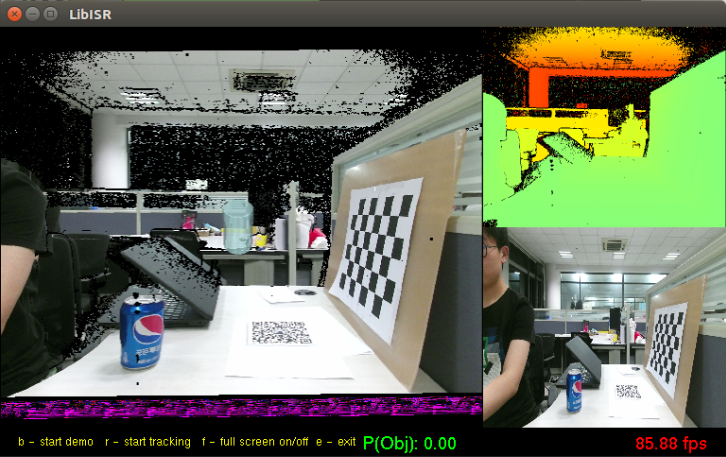
\includegraphics[width=3.3cm]{figure/beforeT.png}
  \hspace{0.1cm}
    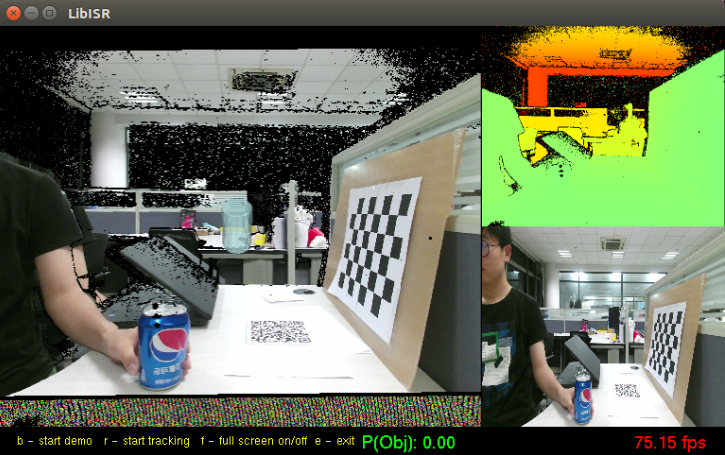
\includegraphics[width=3.3cm]{figure/noT.png}
  \hspace{0.1cm}
    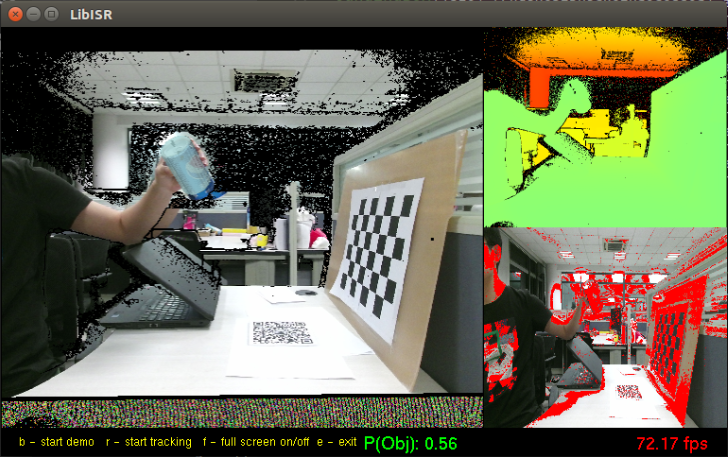
\includegraphics[width=3.3cm]{figure/staticT.png}
  \hspace{0.1cm}
  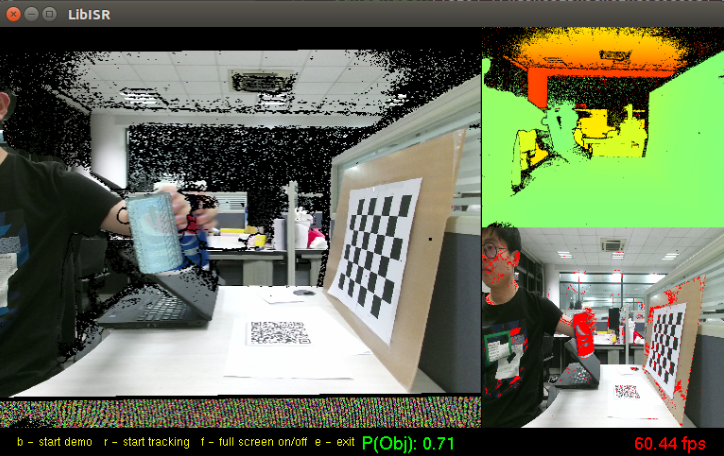
\includegraphics[width=3.3cm]{figure/movingT.png}
  \bicaption[物体追踪不同状态截图]
    {物体追踪不同状态截图}
    {The Screenshots of Tracing Object in Different Situations}
  \label{fig:SRR}
\end{figure}


\begin{figure}[!htp]
  \centering
  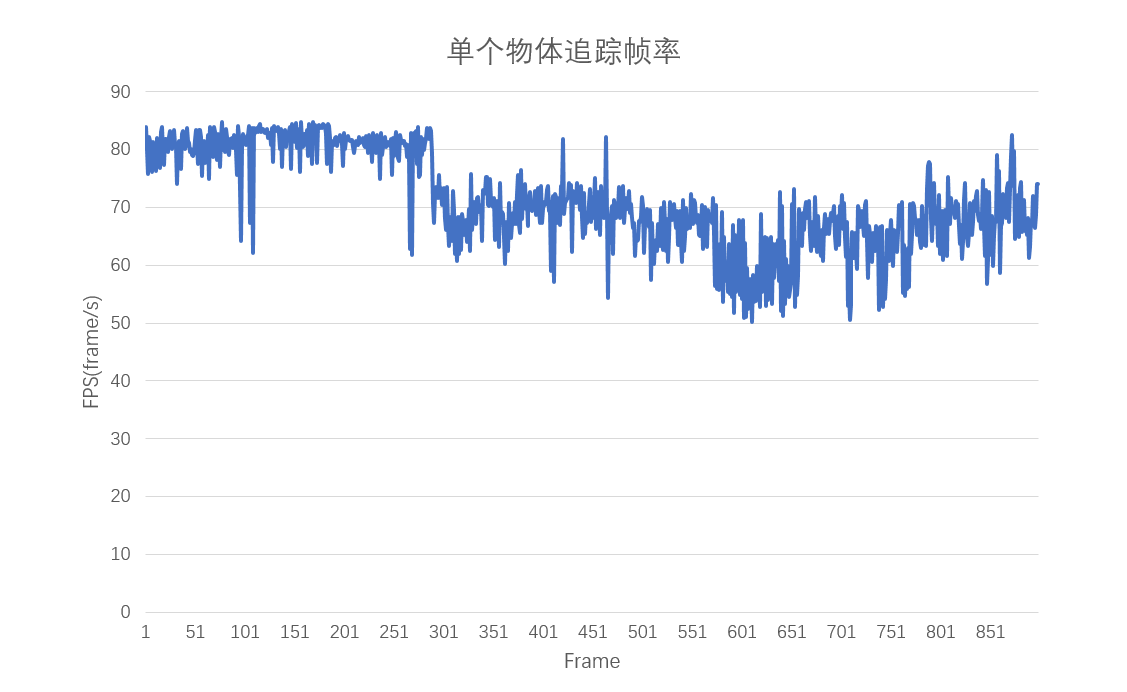
\includegraphics[width=10cm]{figure/fps.png}
  \bicaption[单个物体追踪帧-帧率折线图]
    {单个物体追踪帧-帧率折线图}
    {The Line Chart of Frame - Frame Per Second of Tracing Single Object }
 \label{fig:fps}
\end{figure}

从图中可以看出,在开始追踪之前,即仅测量从Kinect获取视频图像的性能,帧率约为80。从250帧左右开始追踪之后,帧率下降,当物体基本保持静止时或物体并没有被追踪到时,帧率约为70。当第550至650帧时,物体处于移动状态,帧率约为55帧。由此可见,帧率在追踪移动物体的时候性能消耗最大,但整体仍然满足60帧的性能需求。

之后在网络联通的情况下,在检测服务器上述速率的同时,检测客户端获取数据的速率,实际上也就是增强现实应用中物体运动姿态更新的频率。在程序中使用一个计数器,会在每次有数据接收的时候计数,然后每秒进行统计。客户端的运行环境为Intel Core i7 6500U处理器以及AMD Radeon R7 M370显卡。由于客户端和服务器在代码上保证了同步,因此该数据也代表了服务器的数据发送速率。经过测试,网络传输保持在每秒25次,这很大程度上是由于网络传输本身,以及实现的同步收发机制所限制的。此外,也利用Unity中的Coroutine进行每秒统计项目的帧数计算帧率,项目的帧率则被Unity保持在60。

最后,也检测了在移动端应用接受数据的传输速率。手机使用HiSilicon Kirin 970处理器。此时网络通讯速率仍然为每秒25次,项目帧率被Unity锁在30,但是实际上并不影响使用。

\section{交互分析}
系统在PC端和安卓手机端都进行了安装,两者都可以完成预期的工作。

在编著页面,使用手机的过程中,用户可以顺利完成点击、拖动等操作,实现全部预期需求,包括实验环境的修改,实验器具和药品的添加和编辑,实验流程的编辑、实验提示信息属性编辑等。所有的交互方式与PC端保持一致,同时都可以基于手指触摸完成。

在交互页面,用户可以通过手机向服务器发送指令,开始追踪,并且经过标定后,将虚拟物体与真实物体重合并且同步移动。在这个过程中,用户需要用手机拍摄到二维码,之后可以移动物体,观察手机中的虚拟图像。

\section{虚实融合效果分析}

在手机应用中虚拟物体与真实物体的融合效果如图所示,在经过比较精确的标定之后可以有较好的融合效果。